% questions.tex —— 2008 年·普通高等学校招生全国统一考试（四川延期卷）·文科 · 题目内容片段（无答案）
% 由 tools/generate_projects.py 依来源总账自 2008/2008_数学真题_四川延考区文_试题.md 生成，勿手改（改源 MD 后重跑）


\gkpart{一、选择题}

\begin{question}
\gkti{1}设集合 $A=\{-1,0,1\}$，$A$ 的子集中，含有元素 $0$ 的子集共有（　）

（A）$2$ 个

（B）$4$ 个

（C）$6$ 个

（D）$9$ 个

\end{question}
\begin{question}
\gkti{2}函数 $y=\sqrt{1-x}+\lg x$ 的定义域为（　）

（A）$(0,+\infty)$

（B）$(-\infty,1]$

（C）$(-\infty,0)\cup[1,+\infty)$

（D）$(0,1]$

\end{question}
\begin{question}
\gkti{3}$\left(1+\dfrac1x\right)(1+x)^4$ 的展开式中含 $x^2$ 项的系数（　）

（A）$4$

（B）$6$

（C）$10$

（D）$12$

\end{question}
\begin{question}
\gkti{4}不等式 $|x-2|<1$ 的解集为（　）

（A）$\{x\mid 1<x<3\}$

（B）$\{x\mid 0<x<2\}$

（C）$\{x\mid 1<x<2\}$

（D）$\{x\mid 2<x<3\}$

\end{question}
\begin{question}
\gkti{5}已知 $\tan\alpha=\dfrac12$，则 $\dfrac{(\sin\alpha+\cos\alpha)^2}{\cos2\alpha}=$（　）

（A）$2$

（B）$-2$

（C）$3$

（D）$-3$

\end{question}
\begin{question}
\gkti{6}一个三棱锥的底面边长等于一个球的半径，该正三棱锥的高等于这个球的直径，则球的体积与正三棱锥的体积的比值为（　）

（A）$\dfrac{8\sqrt3\pi}3$

（B）$\dfrac{\sqrt3\pi}6$

（C）$\dfrac{\sqrt3\pi}2$

（D）$8\sqrt3\pi$

\end{question}
\begin{question}
\gkti{7}若点 $P(2,0)$ 到双曲线 $\dfrac{x^2}{a^2}-\dfrac{y^2}{b^2}=1$ 的一条渐近线的距离为 $\sqrt2$，则双曲线的离心率为（　）

（A）$\sqrt2$

（B）$\sqrt3$

（C）$2\sqrt2$

（D）$2\sqrt3$

\end{question}
\begin{question}
\gkti{8}在一次读书活动中，一个同学从 $4$ 本不同的科技书和 $2$ 本不同的文艺书中任选 $3$ 本，则所选的书中既有科技书又有文艺书的概率为（　）

（A）$\dfrac15$

（B）$\dfrac12$

（C）$\dfrac23$

（D）$\dfrac45$

\end{question}
\begin{question}
\gkti{9}过点 $(0,1)$ 的直线与圆 $x^2+y^2=4$ 相交于 $A$、$B$ 两点，则 $|AB|$ 的最小值为（　）

（A）$2$

（B）$2\sqrt3$

（C）$3$

（D）$2\sqrt5$

\end{question}
\begin{question}
\gkti{10}已知两个单位向量 $\boldsymbol a$ 与 $\boldsymbol b$ 的夹角为 $\dfrac{\pi}3$，$\boldsymbol a+\lambda\boldsymbol b$ 与 $\lambda\boldsymbol a-\boldsymbol b$ 互相垂直的充要条件是（　）

（A）$\lambda=-\dfrac{\sqrt3}2$ 或 $\lambda=\dfrac{\sqrt3}2$

（B）$\lambda=-\dfrac12$ 或 $\lambda=\dfrac12$

（C）$\lambda=-1$ 或 $\lambda=1$

（D）$\lambda$ 为任意实数

\end{question}
\begin{question}
\gkti{11}设函数 $y=f(x)$（$x\in\mathbf R$）的图像关于直线 $x=0$ 及直线 $x=1$ 对称，且 $x\in[0,1]$ 时，$f(x)=x^2$，则 $f\left(-\dfrac32\right)=$（　）

（A）$\dfrac12$

（B）$\dfrac14$

（C）$\dfrac34$

（D）$\dfrac94$

\end{question}
\begin{question}
\gkti{12}在正方体 $ABCD-A_1B_1C_1D_1$ 中，$E$ 是棱 $A_1B_1$ 的中点，则 $A_1B$ 与 $D_1E$ 所成角的余弦值为（　）

（A）$\dfrac{\sqrt5}{10}$

（B）$\dfrac{\sqrt{10}}{10}$

（C）$\dfrac{\sqrt5}5$

（D）$\dfrac{\sqrt{10}}5$

\end{question}
\gkpart{二、填空题}

\begin{question}
\gkti{13}函数 $y=\mathrm e^{x+1}-1$（$x\in\mathbf R$）的反函数为\gkblank{}。

\end{question}
\begin{question}
\gkti{14}函数 $f(x)=\sqrt3\sin x-\cos^2x$ 的最大值是\gkblank{}。

\end{question}
\begin{question}
\gkti{15}设等差数列 $\{a_n\}$ 的前 $n$ 项和为 $S_n$，且 $S_5=a_5$。若 $a_4\neq0$，则 $\dfrac{a_7}{a_4}=$\gkblank{}。

\end{question}
\begin{question}
\gkti{16}已知 $\angle AOB=90^\circ$，$C$ 为空间中一点，且 $\angle AOC=\angle BOC=60^\circ$。则直线 $OC$ 与 $AOB$ 平面所成角的正弦值为\gkblank{}。

\end{question}
\gkpart{三、解答题}

\begin{question}
\gkti{17}（本小题满分 12 分）

在 $\triangle ABC$ 中，内角 $A$、$B$、$C$ 对边的边长分别是 $a$、$b$、$c$，已知 $a^2+b^2=2b^2$。

（Ⅰ）若 $B=\dfrac{\pi}4$，且 $A$ 为钝角，求内角 $A$ 与 $C$ 的大小；

（Ⅱ）求 $\sin B$ 的最大值。

\end{question}
\begin{question}
\gkti{18}（本小题满分 12 分）

一条生产线上生产的产品按质量情况分为三类：$A$ 类、$B$ 类、$C$ 类。检验员定时从该生产线上任取 $2$ 件产品进行一次抽检，若发现其中含有 $C$ 类产品或 $2$ 件都是 $B$ 类产品，就需要调整设备，否则不需要调整。已知该生产线上生产的每件产品为 $A$ 类品、$B$ 类品和 $C$ 类品的概率分别为 $0.9$、$0.05$ 和 $0.05$，且各件产品的质量情况互不影响。

（Ⅰ）求在一次抽检后，设备不需要调整的概率；

（Ⅱ）若检验员一天抽检 $3$ 次，求一天中至少有一次需要调整设备的概率。

\Needspace{0.4\textheight}
\end{question}
\begin{question}
\gkti{19}（本小题满分 12 分）

如图，一张平行四边形的硬纸片 $ABC_0D$ 中，$AD=BD=1$，$AB=\sqrt2$。沿它的对角线 $BD$ 把 $\triangle BDC_0$ 折起，使点 $C_0$ 到达平面 $ABC_0D$ 外点 $C$ 的位置。

（Ⅰ）证明：平面 $ABC_0D\perp$ 平面 $CBC_0$；

（Ⅱ）当二面角 $A-BD-C$ 为 $120^\circ$ 时，求 $AC$ 的长。
\nopagebreak[4]
\begin{center}% 2008 年四川延考区卷文科第 19 题：平行四边形硬纸片 ABC0D（AD=BD=1，AB=√2）沿对角线 BD
%   把 △BDC0 折起，C0 到平面 ABC0D 外点 C 的位置。
% 来源 PDF：gaokaomath-src/普通高考/2008/2008延考区文.pdf
% SHA-256：fdfb4e9e88d4405f8a99380d6f2197f3269e061ef9b2c4f7ed7066a56a1e88c2
% 原页：2008延考区文.pdf 第 3 页（A4 单栏），题面第 19 题的配图。
% 绘图方式：取 B(0,0,0)、D(1,0,0)、A(1,1,0)、C0(0,-1,0)（平面 ABC0D 为 z=0），
%   把 C0 绕 BD 折起 60°，得 C(0,-0.5,0.866)；屏幕投影取 (x+0.35y, 0.95z+0.5y)，缩放 2 倍后平移。
%   实线为折起后可见的棱 AB、AD、BD、BC、DC；虚线为 C0 所在的原位置 BC0、DC0。
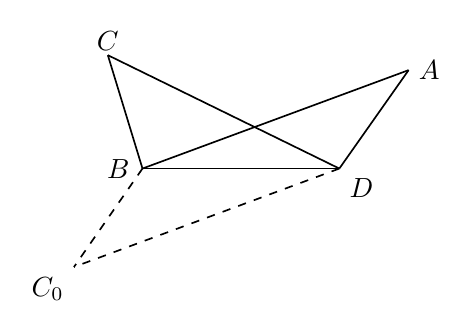
\begin{tikzpicture}[scale=1.0, semithick, every node/.style={inner sep=1.4pt}]
  \coordinate (B) at (1.30,1.40);
  \coordinate (D) at (3.80,1.40);
  \coordinate (A) at (4.68,2.65);
  \coordinate (C0) at (0.43,0.15);
  \coordinate (C) at (0.86,2.84);

  % 折起后可见的棱
  \draw (A) -- (B);
  \draw (A) -- (D);
  \draw (B) -- (D);
  \draw (B) -- (C);
  \draw (D) -- (C);

  % 折起前 C0 所在的原位置
  \draw[dashed] (B) -- (C0);
  \draw[dashed] (D) -- (C0);

  \node[right=2pt] at (A) {$A$};
  \node[left=3pt] at (B) {$B$};
  \node[below right=2pt] at (D) {$D$};
  \node[below left=2pt] at (C0) {$C_0$};
  \node[above] at (C) {$C$};
\end{tikzpicture}
\end{center}
\nopagebreak[4]
\end{question}
\begin{question}
\gkti{20}（本小题满分 12 分）

在数列 $\{a_n\}$ 中，$a_1=1$，$2a_{n+1}=\left(1+\dfrac1n\right)^2a_n$。

（Ⅰ）证明数列 $\left\{\dfrac{a_n}{n^2}\right\}$ 是等比数列，并求 $\{a_n\}$ 的通项公式；

（Ⅱ）令 $b_n=a_{n+1}-\dfrac12a_n$，求数列 $\{b_n\}$ 的前 $n$ 项和 $S_n$；

（Ⅲ）求 $\{a_n\}$ 的前 $n$ 项和 $T_n$。

\end{question}
\begin{question}
\gkti{21}（本小题满分 12 分）

已知椭圆 $C_1$ 的中心和抛物线 $C_2$ 的顶点都在坐标原点 $O$，$C_1$ 和 $C_2$ 有公共焦点 $F$，点 $F$ 在 $x$ 轴上，且 $C_1$ 的长半轴上，且 $C_1$ 的长轴长、短轴长及点 $F$ 到 $C_1$ 右准线的距离成等比数列。

（Ⅰ）当 $C_2$ 的准线与 $C_1$ 右准线间的距离为 $15$ 时，求 $C_1$ 及 $C_2$ 的方程；

（Ⅱ）设过点 $F$ 且斜率为 $1$ 的直线 $l$ 交 $C_1$ 于 $P$、$Q$ 两点，交 $C_2$ 于 $M$、$N$ 两点，当 $|MN|=8$ 时，求 $|PQ|$ 的值。

\end{question}
\begin{question}
\gkti{22}（本小题满分 14 分）

设函数 $f(x)=x^3-x^2-x+2$。

（Ⅰ）求函数 $f(x)$ 的单调区间和极值；

（Ⅱ）当 $x\in[-1,2]$ 时，$-3\leqslant af(x)+b\leqslant3$，求 $a-b$ 的最大值。

\end{question}